\chapter{Computational Study}

This chapter presents our computational study and is structured as follows: Section 5.1 describes the data our experiments are conducted on.  
\section{Data description}

The available data set is provided by \cite{Hildebrandt2020_EAT} who created a high-dimensional data model with the RMDP instances originally used in \cite{UlmerRMDP}. It comprises 850.469 samples, 23.341 unique customer locations and 15 unique restaurant locations, latter being the result of a 15-medoid clustering of originally 110 restaurants contained in the RMDP instances. The temporal and spatial distribution of the orders is depicted in figure \ref{fig:dists}. 
\begin{figure}[h]
	\centering
	\subfigure[Spatial distributions]{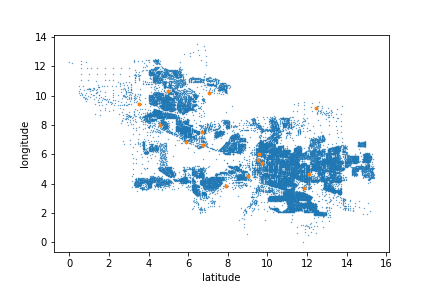
\includegraphics[width=0.49\linewidth]{../Implementation/Plots/spatial_dist.png}}
	\subfigure[Temporal distributions]{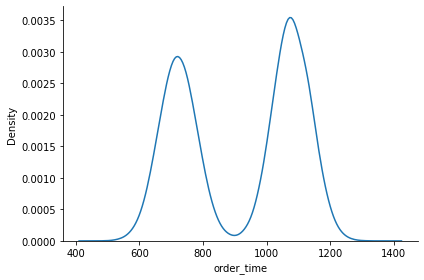
\includegraphics[width=0.49\linewidth]{../Implementation/Plots/order_time_dist.png}}
	\caption{Spatial and temporal distributions}
	\label{fig:dists}
\end{figure}

The temporal distribution depicted in the right panel of figure \ref{fig:dists} shows that the order behaviour across all customers follows a bimodal gaussian distribution. The x-axis represents the day time at which the orders took place, while the y-axis shows how many customer ordered at a certain day time.
 
\section{Parametrization of Methods}

\section{Results}







